\documentclass[aspectratio=169]{beamer}

% ---------- Ocean Blue & Amber Theme ----------
\usepackage[utf8]{inputenc}
\usepackage{tikz}
\usetikzlibrary{positioning,arrows.meta,shapes}
\usepackage{graphicx}
\usepackage{booktabs}
\usepackage{array}
\usepackage{colortbl}

\definecolor{oceanblue}{RGB}{9,54,96}
\definecolor{oceanblueLight}{RGB}{28,99,161}
\definecolor{amber}{RGB}{255,176,0}
\definecolor{amberDark}{RGB}{204,133,0}
\definecolor{offwhite}{RGB}{247,249,251}

\setbeamercolor{normal text}{fg=oceanblue,bg=offwhite}
\setbeamercolor{structure}{fg=oceanblue}
\setbeamercolor{palette primary}{bg=oceanblue,fg=white}
\setbeamercolor{palette secondary}{bg=oceanblueLight,fg=white}
\setbeamercolor{palette tertiary}{bg=amber,fg=oceanblue}
\setbeamercolor{title}{fg=white}
\setbeamercolor{frametitle}{bg=oceanblue,fg=white}
\setbeamercolor{block title}{bg=amber,fg=oceanblue}
\setbeamercolor{block body}{bg=amber!12,fg=oceanblue}
\setbeamercolor{item}{fg=amberDark}
\setbeamercolor{footline}{fg=white,bg=oceanblue}

\setbeamertemplate{navigation symbols}{}
\setbeamertemplate{itemize item}{\color{amberDark}\textbullet}
\setbeamertemplate{itemize subitem}{\color{oceanblueLight}\textendash}
\setbeamerfont{frametitle}{series=\bfseries}

\setbeamertemplate{footline}{
  \leavevmode
  \hbox{\begin{beamercolorbox}[wd=\paperwidth,ht=2.5ex,dp=1ex,leftskip=1em,rightskip=1em]{footline}
  \small \insertshorttitle \hfill \insertframenumber/\inserttotalframenumber
  \end{beamercolorbox}}
}

\title{RoboSoccer: Bluetooth-Controlled Soccer Robots}
\subtitle{Project Proposal}
\author{\color{white}
Arjo Kar (ID: 2205031)\\
Sanjoy Kumar Shuvo (ID: 2205035)\\
Zannatun Nayeem Ohee (ID: 2205059)
}

\date{\today}

% ---------- Reusable equipment-slide layout ----------
\newcommand{\equipslide}[3]{%
  \begin{frame}{Equipment -- #1}
    #2
    \vspace{0.4cm}
    \begin{center}
      \includegraphics[width=0.42\linewidth,height=5cm,keepaspectratio]{#3}
    \end{center}
  \end{frame}
}

\begin{document}

% ---------- Title Page ----------
\begin{frame}[plain]
  \begin{tikzpicture}[remember picture, overlay]
    \fill[oceanblue] (current page.south west) rectangle (current page.north east);
    \fill[amber] ([yshift=1.4cm]current page.south west) rectangle ([yshift=1.55cm]current page.south east);

    \node[align=center, text width=11cm] at ([yshift=1.1cm]current page.center) {
      {\fontsize{28}{30}\selectfont\color{white}\bfseries RoboSoccer}\\[0.2cm]
      {\Large\color{amber} Bluetooth-Controlled Soccer Robots}\\[0.35cm]
      {\large\color{white!75!oceanblue} Project Proposal}
    };

    \node[align=center, text width=11cm] at ([yshift=-1.6cm]current page.center) {
      \small\color{white!85!oceanblue}
      Arjo Kar \textcolor{amber}{|} 2205031 \\[0.15cm]
      Sanjoy Kumar Shuvo \textcolor{amber}{|} 2205035 \\[0.15cm]
      Zannatun Nayeem Ohee \textcolor{amber}{|} 2205059
    };

    \node[align=center, font=\scriptsize] at ([yshift=1.1cm]current page.south) {
      \color{white!70!oceanblue}
    };
  \end{tikzpicture}
\end{frame}

% ---------- Motivation ----------
\begin{frame}{Motivation}
  \begin{block}{Why This Project}
    With the FIFA World Cup 2026 around the corner, football fever is everywhere --
    and we wanted to bring that same excitement into our lab. Instead of another
    routine sensor-and-motor exercise, we chose to build something we would
    genuinely enjoy designing, testing, and playing with.
  \end{block}
  \begin{itemize}
    \item \textbf{Entertainment \& refreshment}: a physical, competitive game
          that turns lab time into something fun rather than another checklist task.
    \item \textbf{Inspired by FIFA WC 2026}: the global excitement around football
          this year directly shaped our choice of a soccer-robot theme.
    \item \textbf{Hands-on learning}: still exercises core embedded concepts
          (UART, PWM, timers, interrupts) -- just wrapped in a project we're
          actually excited to finish.
  \end{itemize}
\end{frame}

\begin{frame}{Objectives}
  \begin{itemize}
    \item Design two independent 4-wheel drive robot cars, each controlled by a mobile app over Bluetooth.
    \item Implement smooth motor control using PWM through TB6612FNG drivers.
    \item Add a kicker mechanism using a servo motor.
    \item Implement a laser-based goal detection system at each goalpost.
    \item Demonstrate a complete two-player robo-soccer match as final deliverable.
  \end{itemize}
\end{frame}

% ---------- Equipment (one slide per component) ----------
\equipslide{ATmega32}{
  Main microcontroller, motor \& servo control, sensor input.
}{images/atmega32.jpeg}

\equipslide{HC-05 Bluetooth Module}{
  Receives drive/kick commands from the Android app.
}{images/hc05.jpeg}

\equipslide{TB6612FNG Motor Driver}{
  Drives the 4 DC motors (left pair / right pair).
}{images/TB6612FNG.jpeg}

\equipslide{6V Geared DC Motors, TT-type}{
  Drive the robot's wheels.
}{images/dc_motor.png}

\equipslide{Servo Motor, SG90/MG90S/MG996R}{
  Rotates the kicking arm to shoot the ball.
}{images/servo.png}

\equipslide{Robot Chassis + Wheels}{
  Base frame and locomotion.
}{images/chassis.png}

\begin{frame}{Equipment -- Additional Components}
  \begin{itemize}
    \item \textbf{Servo Horn \& Screws, Kicking Arm} -- converts servo rotation into a kicking strike.
    \item \textbf{U-shaped Ball Holder} -- holds the ball in front of the robot before the kick.
    \item \textbf{Breadboard \& Jumper Wires}
    \item \textbf{Laser Module + Laser Receiver} -- detects ball crossing the goal line.
  \end{itemize}
\end{frame}

\begin{frame}{Equipment -- Software / Tools}
  \begin{itemize}
    \item \textbf{Atmel Studio / AVR-GCC} -- firmware development for ATmega32.
    \item \textbf{AVRDUDE} -- flashing the microcontroller.
    \item \textbf{Proteus} -- circuit simulation and PCB layout.
    \item \textbf{Mobile App} -- For Bluetooth control.
  \end{itemize}
\end{frame}

% ---------- System Design ----------
\begin{frame}{System Design -- Control Connections}
  \centering
  \resizebox{0.95\linewidth}{!}{%
  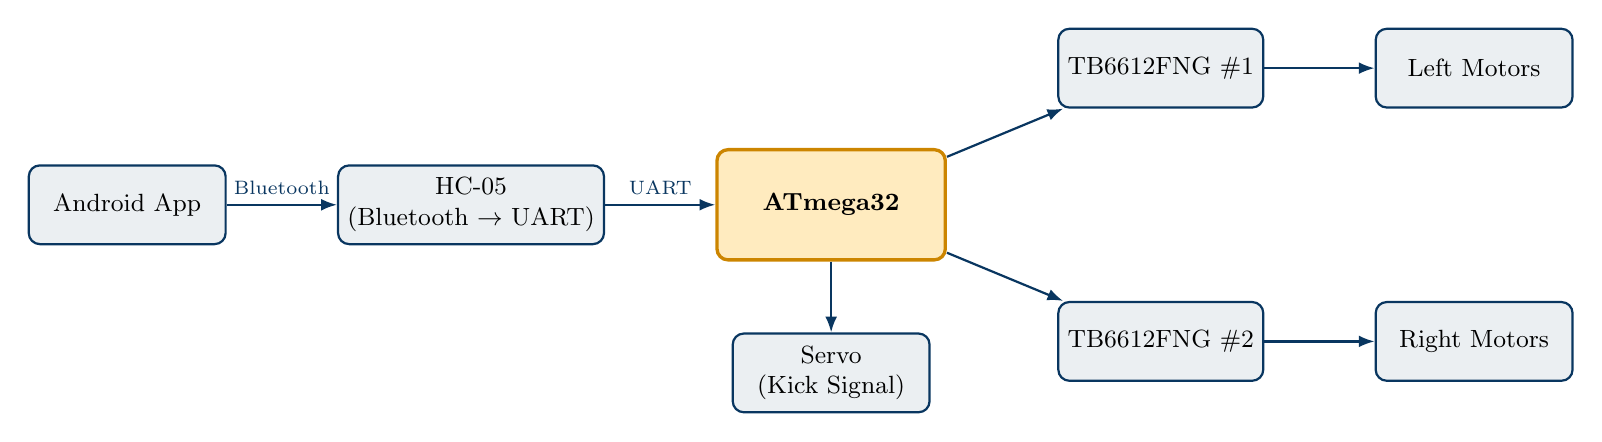
\begin{tikzpicture}[
      node distance=1.0cm and 1.4cm,
      block/.style={rectangle, draw=oceanblue, thick, fill=oceanblue!8,
                    rounded corners, minimum height=1cm, minimum width=2.5cm,
                    align=center, font=\small},
      mcu/.style={rectangle, draw=amberDark, very thick, fill=amber!25,
                  rounded corners, minimum height=1.4cm, minimum width=2.9cm,
                  align=center, font=\bfseries\small},
      arrow/.style={-{Latex[length=2mm]}, thick, oceanblue}
    ]
    % --- Car unit (representative of both cars) ---
    \node[block] (app) {Android App};
    \node[block, right=of app] (hc05) {HC-05\\(Bluetooth $\to$ UART)};
    \node[mcu, right=of hc05] (mcu) {ATmega32};
    \node[block, above right=0.5cm and 1.4cm of mcu] (drv1) {TB6612FNG \#1};
    \node[block, below right=0.5cm and 1.4cm of mcu] (drv2) {TB6612FNG \#2};
    \node[block, right=1.4cm of drv1] (m1) {Left Motors};
    \node[block, right=1.4cm of drv2] (m2) {Right Motors};
    \node[block, below=0.9cm of mcu] (servo) {Servo\\(Kick Signal)};

    \draw[arrow] (app) -- node[above,font=\scriptsize]{Bluetooth} (hc05);
    \draw[arrow] (hc05) -- node[above,font=\scriptsize]{UART} (mcu);
    \draw[arrow] (mcu) -- (drv1);
    \draw[arrow] (mcu) -- (drv2);
    \draw[arrow] (drv1) -- (m1);
    \draw[arrow] (drv2) -- (m2);
    \draw[arrow] (mcu) -- (servo);

    
  \end{tikzpicture}}
  \vspace{0.2cm}\\
\end{frame}

\begin{frame}{System Design -- Component Roles}
  \begin{itemize}
    \item \textbf{Android App}: sends drive/kick commands over Bluetooth serial.
    \item \textbf{HC-05}: wireless UART bridge to ATmega32.
    \item \textbf{ATmega32}: decodes commands, generates PWM, manages sensor interrupts.
    \item \textbf{TB6612FNG}: converts PWM + direction signals into motor drive current.
    \item \textbf{DC Motors}: provide locomotion for the 4-wheel chassis.
    \item \textbf{Servo + Kicking Arm}: strikes the ball on command.
    \item \textbf{Laser + Receiver}: detects the ball breaking the beam at the goal mouth.
    \item \textbf{2S Battery + BMS}: raw power source with charge/discharge protection.
    \item \textbf{LM2596}: regulated 5V supply for ATmega32, HC-05, and (5V) servo.
    \item \textbf{Main Switch}: master on/off for the whole system.
  \end{itemize}
\end{frame}

\begin{frame}{Key ATmega32 Pins / Interfaces}
  \begin{itemize}
    \item \textbf{UART (RXD/TXD)}: serial link to HC-05 for app commands.
    \item \textbf{Timer0/Timer1 PWM (OC0, OC1A/OC1B)}: speed control for drive motors and servo signal.
    \item \textbf{GPIO Port A/B}: direction control pins (AIN1/AIN2, BIN1/BIN2) for TB6612FNG.
    \item \textbf{External Interrupt (INT0/INT1)}: goal-detection trigger from laser receiver.
    \item \textbf{ADC channel}: battery voltage monitoring (optional).
  \end{itemize}
\end{frame}

\begin{frame}{Software Features -- Command Protocol}
  \begin{block}{App Layout}
    The Android app has six buttons; each press sends a single ASCII character
    over Bluetooth, which the ATmega32 receives via UART and maps to an action.
  \end{block}
  \small
  \begin{tabular}{@{}p{2.3cm}p{1.2cm}p{7.5cm}@{}}
    \toprule
    \textbf{Button} & \textbf{Char} & \textbf{ATmega32 Action} \\
    \midrule
    Forward  & F & Both drivers forward, equal PWM duty. \\
    Backward & B & Both drivers reverse, equal PWM duty. \\
    Left     & L & Left motors reverse / right motors forward (or reduced left speed). \\
    Right    & R & Right motors reverse / left motors forward (or reduced right speed). \\
    Stop     & S & All motor PWM set to 0. \\
    Kick     & K & Servo sweeps to kick angle, then returns to rest. \\
    \bottomrule
  \end{tabular}
\end{frame}

% ---------- Role of ATmega32 ----------
\begin{frame}{Role of the ATmega32}
  \begin{block}{Core Responsibilities}
    The ATmega32 is the central controller for each car -- it is not a passive
    relay but performs all real-time decision making and actuation.
  \end{block}
  \begin{itemize}
    \item Parses Bluetooth commands received via UART from the HC-05 module.
    \item Generates PWM signals (Timer0/Timer1) to control 4 drive motors through two TB6612FNG drivers.
    \item Generates a separate PWM signal to position the servo-driven kicker.
    \item Uses external interrupts to instantly detect a goal event from the laser receiver.
    \item Uses GPIO pins to set motor direction (forward/reverse/turn logic).
    \item Optionally uses ADC to monitor battery voltage and trigger a low-battery alert.
  \end{itemize}
\end{frame}

% ---------- Implementation Plan ----------
\begin{frame}{Implementation Plan -- Expected Outcome}
  \begin{block}{Final Outcome}
    Two independently Bluetooth-controlled 4-wheel robot cars capable of
    driving, kicking a ball, and automatically detecting goals via a
    laser-beam sensor -- forming a complete two-player robo-soccer match.
  \end{block}
\end{frame}

\begin{frame}{Implementation Plan -- 5 Week Timeline}
  \small
  \begin{tabular}{@{}p{1.6cm}p{9.7cm}}
    \toprule
    \textbf{Week} & \textbf{Milestone} \\
    \midrule
    Week 1 & Component procurement, chassis assembly, basic ATmega32 + motor driver testing. \\
    Week 2 & HC-05 Bluetooth interfacing, UART command protocol design, Mobile App configuration \\
    \rowcolor{amber!25} Week 3 & \textbf{Project Update 1}: single car drives via app control (forward/back/turn) with PWM speed control. \\
    Week 4 & Servo kicker integration, laser goal-detection module testing, dual-car synchronization. \\
    \rowcolor{amber!25} Week 5 & \textbf{Final Submission}: full two-car match demo, goal detection, bug fixing, documentation. \\
    \bottomrule
  \end{tabular}
\end{frame}

\begin{frame}{Milestones \& Dependencies}
  \begin{itemize}
    \item Motor driver testing depends on chassis assembly being complete.
    \item Bluetooth command protocol must be finalized before app development.
    \item Goal detection integration depends on laser module calibration.
    \item Final demo depends on both cars being functionally independent and tested together.
  \end{itemize}
\end{frame}

% ---------- Other Controllers ----------
\begin{frame}{Use of Other Controllers}
  \begin{block}{Note}
    This project does not require an additional microcontroller (e.g. ESP32,
    Arduino, Raspberry Pi). The ATmega32 alone handles motor control, servo
    actuation, Bluetooth communication, and goal-detection.
  \end{block}

\end{frame}

% ---------- Testing and Success Criteria ----------
\begin{frame}{Testing Strategy}
  \begin{itemize}
    \item Unit test each module individually: motor driver response, servo angle accuracy, Bluetooth range/latency.
    \item Integration testing: full command-to-motion latency measurement.
    \item Field testing: goal-detection reliability under different lighting/ball speeds.
    \item Stress testing: continuous operation time on battery power.
  \end{itemize}
\end{frame}

\begin{frame}{Success Criteria}
  \begin{columns}[T]
    \begin{column}{0.5\textwidth}
      \textbf{Essential (Must-Have)}
      \begin{itemize}
        \item Reliable Bluetooth control of both cars.
        \item Smooth forward/reverse/turn motion via PWM.
        \item Functional servo kicker.
        \item Accurate goal detection via laser sensor.
      \end{itemize}
    \end{column}
    \begin{column}{0.5\textwidth}
      \textbf{Optional (Nice-to-Have)}
      \begin{itemize}
        \item Battery-level monitoring and alert.
        \item Score display/counter.
        \item Adjustable motor speed profiles.
        \item LED indicators for game status.
      \end{itemize}
    \end{column}
  \end{columns}
\end{frame}

% ---------- Challenges and Future Scope ----------
\begin{frame}{Challenges}
  \begin{itemize}
    \item Ensuring low-latency, interference-free dual Bluetooth links during simultaneous play.
    \item Precise motor speed matching for straight-line driving (motor tolerance variation).
    \item Reliable laser-receiver triggering under ambient light interference.
    \item Power budget management for motors, servo, and logic on a single 2S battery pack.
  \end{itemize}
\end{frame}

\begin{frame}{Future Scope}
  \begin{itemize}
    \item Implement autonomous ball detection and tracking using a camera or vision sensor.
    \item Add obstacle detection and avoidance using ultrasonic or infrared sensors.
    \item Integrate wheel encoders for accurate speed and distance control.
    \item Upgrade to a custom PCB to improve reliability and reduce wiring complexity.
    \item Improve the kicking mechanism using a solenoid or spring-loaded actuator for stronger shots.
  \end{itemize}
\end{frame}

% ---------- Thank You ----------
\begin{frame}[plain]
  \begin{tikzpicture}[remember picture, overlay]
    \fill[oceanblue] (current page.south west) rectangle (current page.north east);
    \fill[amber] ([yshift=-1.4cm]current page.north west) rectangle ([yshift=-1.55cm]current page.north east);

    \node[align=center, text width=11cm] at (current page.center) {
      {\Huge \color{white} \textbf{Thank You}}\\[0.35cm]
    };
  \end{tikzpicture}
\end{frame}

\end{document}